\documentclass[tikz,border=3pt]{standalone}
\usepackage{pgfplots}
\usepgfplotslibrary{groupplots}
\pgfplotsset{compat=1.18}
\begin{document}
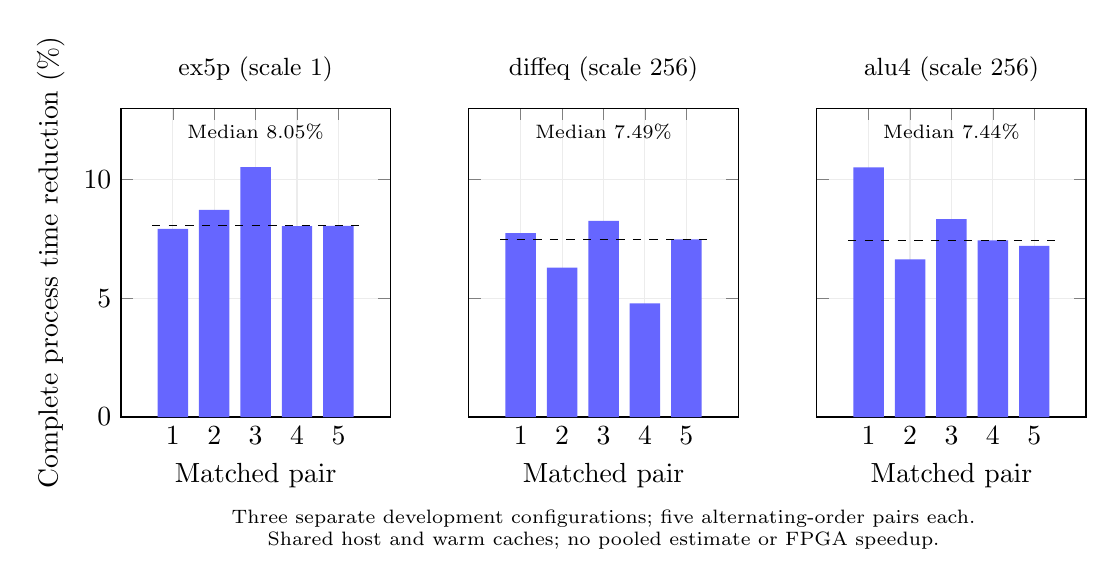
\begin{tikzpicture}
\begin{groupplot}[group style={group size=3 by 1,horizontal sep=1cm},width=5cm,height=5.5cm,xlabel={Matched pair},xtick={1,2,3,4,5},ymin=0,ymax=13,enlarge x limits=.15,grid=major,grid style={gray!15},title style={font=\small}]
\nextgroupplot[ylabel={Complete process time reduction (\%)},title={ex5p (scale 1)}]
\addplot[ybar,/pgf/bar width=11pt,fill=blue!60,draw=none] coordinates {(1,7.92423847) (2,8.72929029) (3,10.53135334) (4,8.04525812) (5,8.05425156)};
\addplot[black,dashed,domain=.5:5.5] {8.054251556719693};
\node[anchor=north,font=\scriptsize] at (rel axis cs:.5,.98) {Median 8.05\%};
\nextgroupplot[yticklabels={},title={diffeq (scale 256)}]
\addplot[ybar,/pgf/bar width=11pt,fill=blue!60,draw=none] coordinates {(1,7.74759259) (2,6.28969678) (3,8.26555555) (4,4.78790910) (5,7.48703297)};
\addplot[black,dashed,domain=.5:5.5] {7.487032970578089};
\node[anchor=north,font=\scriptsize] at (rel axis cs:.5,.98) {Median 7.49\%};
\nextgroupplot[yticklabels={},title={alu4 (scale 256)}]
\addplot[ybar,/pgf/bar width=11pt,fill=blue!60,draw=none] coordinates {(1,10.51527907) (2,6.64559481) (3,8.33913515) (4,7.43989451) (5,7.21617042)};
\addplot[black,dashed,domain=.5:5.5] {7.43989450865663};
\node[anchor=north,font=\scriptsize] at (rel axis cs:.5,.98) {Median 7.44\%};
\end{groupplot}
\node[anchor=north,font=\scriptsize,align=center,yshift=-30pt] at (group c2r1.south) {Three separate development configurations; five alternating-order pairs each.\\Shared host and warm caches; no pooled estimate or FPGA speedup.};
\end{tikzpicture}
\end{document}
